\documentclass[tikz,border=6pt]{standalone}
\usepackage[T1]{fontenc}
\usepackage{helvet}
\renewcommand{\familydefault}{\sfdefault}
\usetikzlibrary{arrows.meta,fit}
\tikzset{
  box/.style={draw,thick,minimum width=3.6cm,minimum height=1.2cm,align=center,font=\small},
  arr/.style={-{Stealth[length=2.5mm]},thick},
  biarr/.style={{Stealth[length=2.5mm]}-{Stealth[length=2.5mm]},thick}
}
\begin{document}
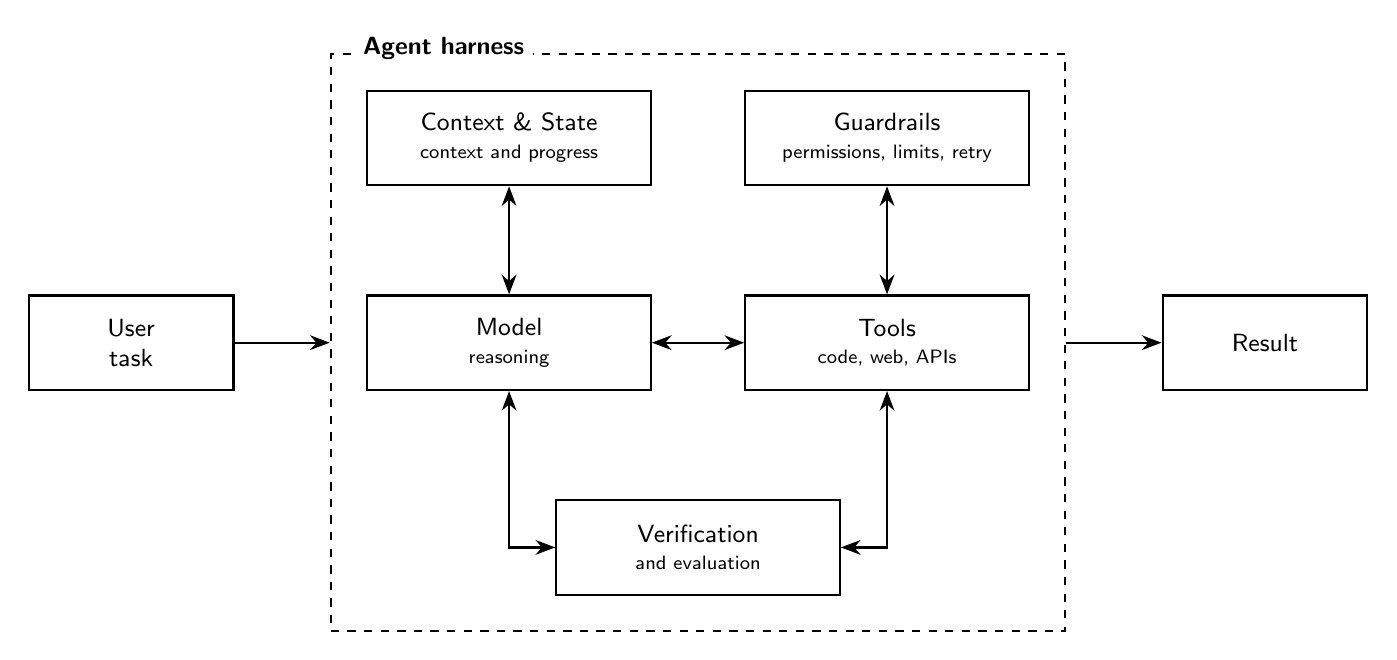
\begin{tikzpicture}
  \node[box] (model) at (0,0) {Model\\[-1pt]{\scriptsize reasoning}};
  \node[box] (tools) at (4.8,0) {Tools\\[-1pt]{\scriptsize code, web, APIs}};
  \node[box] (ctx) at (0,2.6) {Context \& State\\[-1pt]{\scriptsize context and progress}};
  \node[box] (guard) at (4.8,2.6) {Guardrails\\[-1pt]{\scriptsize permissions, limits, retry}};
  \node[box] (ver) at (2.4,-2.6) {Verification\\[-1pt]{\scriptsize and evaluation}};

  \draw[biarr] (model) -- (tools);
  \draw[biarr] (ctx) -- (model);
  \draw[biarr] (guard) -- (tools);
  \draw[biarr] (model.south) |- (ver.west);
  \draw[biarr] (tools.south) |- (ver.east);

  \node[draw,thick,dashed,inner sep=0.45cm,fit=(model)(tools)(ctx)(guard)(ver)] (h) {};
  \node[font=\bfseries\small,fill=white,anchor=south west] at ([xshift=0.3cm,yshift=-0.2cm]h.north west) {Agent harness};

  \node[box,minimum width=2.6cm] (user) at (-4.8,0) {User\\task};
  \node[box,minimum width=2.6cm] (res) at (9.6,0) {Result};
  \draw[arr] (user) -- (user -| h.west);
  \draw[arr] (h.east |- res) -- (res);
\end{tikzpicture}
\end{document}
